\chapter{Orbital dynamics around Asteroids}
\label{chap:dynamics_modeling}
\graphicspath{{Modeling/Images/}}

This chapter will focus on accurate modeling of the asteroid environment and the equations of motion of a particle around it in presence of gravitational and Solar perturbations.

\section{Modeling Assumptions}
\label{sec:assumptions}
The simulator designed as part of this research (see \Cref{chap:naos}) involves some degree of approximation of the real-world dynamical environment around the asteroid. Every degree-of-freedom and complexity added to a simulator to resemble the real-world, will also act as a potential source of error. By designing a relatively simpler simulator, we can explain the characteristic behavior of regolith through fundamentals while keeping the sources of error to as low as possible. Ofcourse, we verify the simulator (see \Cref{chap:v_and_v}) but by including a higher degree of fidelity in the simulator, we increase the workload on the verification process as well, thereby reducing the scientific output in the end. Moreover, the current simulator and the results from it will act as a benchmark for a higher-fidelity simulator in the future. Thus, the approximations made in this thesis are mentioned as follows:
% Every research involves some degree of approximation of the natural world, on Earth or otherwise, to understand or explain any phenomenon. Through this thesis work, we hope to understand the orbital behavior of regolith around an asteroid and we have to do it with a relatively simplified model because recreating an exact replica of an asteroid's dynamical environment is out of the scope of this thesis. Although we are making simplifications, but it does not mean that the scientific returns from it would be any less. The particle trajectories might not be exact when we conduct the simulation based experiments in real world but the underlying science explaining the orbital behavior would remain unchanged (this would become more clear in \Cref{chap:results}). Thus, the simplifying assumptions we make for modeling the asteroid-regolith system are mentioned as follows:
%%%
\begin{enumerate}
\item The asteroid body is modeled as a smooth triaxial ellipsoid to account for its non-uniform gravity. The reasons for choosing this model over others will be explained later in \Cref{sec:gravity}.

\item Craters, surface depressions, mountains or any other terrain deformity on the asteroid is not considered in the simulation. The body is considered to have a uniform density. This is to simplify calculations of the gravitational acceleration.

\item The asteroid is rotating uniformly about its shortest axis. This is considered for simplicity and also because most Solar System bodies would dissipate energy to eventually enter a rotational state that is uniform and about its axis of maximum moment of inertia \parencite{scheeresBook}. Hence, the approximation for the asteroid remains valid.

\item The regolith grains are assumed to be spherical in shape to simplify the \gls{SRP} calculation as the cross-sectional area of a sphere would remain the same irrespective of its attitude.

\item Multiple regolith particles are launched from a given location on the asteroid in the form of a cone to replicate ejecta from a cratering event. But all particles are assumed to be coming off from the same point, unlike that in the case of an actual cratering event. This is because the pretext of the thesis was that the regolith is lofted due to an activity from a spacecraft and such would result in relatively smaller craters (from artificial cratering events) or surface depressions. Thus assuming that all particles in this \textit{"ejecta cone"} emerge from the same point on the asteroid is reasonable and simplifies the simulation.

\item The slant angle of the \textit{"ejecta cone"} (henceforth the declination angle) from the local surface normal is kept constant at 45.0 [deg] (which is a middle value in the entire declination range from 0.0 - 90.0 [deg]). We want to consider a general case and not introduce another degree-of-freedom in terms of varying declination angles.

\item The loss of material and mass from the asteroid, when the regolith is lofted from the surface, is not modeled in the simulation since it is assumed that a very small amount of material will be displaced by a spacecraft activity. This assumption is based on the sample collected by the Hayabusa mission (see \Cref{sec:past_missions} and the references therein).

\item Interaction between individual regolith grain is not accounted for because we are simulating multiple particles being lofted at the same time and granular interaction on such a scale would be extremely complex and beyond the scope of this thesis.

\item Secondary motion of regolith, after re-impacting the surface is not modeled and it is assumed that the particles just come to a standstill.

\item The shadow region of the asteroid is not modeled which means that the solar perturbations are always acting on the regolith grain and this simplification was made since asteroids are extremely small compared to planets, and thus the orbiting particles wouldn't spend long periods of time in the shadow.

\item Perturbations are considered only from the Sun. \gls{SRP} is important because regolith grains will have higher Area-To-Mass ratios, relative to a spacecraft, and so the radiation pressure would be significantly large for them. We model the third body attraction from the Sun (\gls{STBE}) as well but not from any of the giant planets such as Jupiter or Saturn, because the magnitude of perturbation from the \gls{STBE} itself is atleast 5 orders of magnitude smaller than the gravitational acceleration when the regolith is in close proximity to the asteroid (see \Cref{chap:results}).

\item The apparent motion of the Sun around the asteroid is considered circular and in the equatorial plane of the asteroid and this was based on the orbital element measurements of all observed asteroids. Majority of these asteroids have small orbital eccentricities \parencite{malhotra2016_eccentricityDistribution}, quite a few of which have a nearly circular orbit. \cite{jedicke1998_orbitalElements} presents debiased measurements for the inclination of the \gls{MBO} and shows that a large number of asteroids have near-zero inclinations.
\end{enumerate}
%%%

\section{Reference Frames}
\label{sec:reference_frames}
Before describing the motion of regolith around the asteroid, its important to define the frames of reference with respect to which this motion is defined and the transformation of state vectors between these frames. We use two asteroid centric reference frames, both of which are depicted in \Cref{fig:reference_frame}. Since we will be using a triaxial ellipsoid to model an asteroid (for details, see \Cref{sec:gravity}), the body-fixed rotating frame and the inertial frame with respect to this model are shown in \Cref{fig:ellipsoid_rotating_frame,fig:solar_phase_and_inertial_frame} respectively.
%%%
\begin{figure}[htb]
\centering
\captionsetup{justification=centering}
\includegraphics[width=\textwidth, height=0.35\textheight, keepaspectratio=true]{reference_frames.pdf}
\caption{The diagram depicts two asteroid centric reference frames, one being Inertial (depicted by solid line and the subscript \emph{I}) and the other being a body-fixed Rotating frame (denoted by dashed line and the subscript \emph{B}). The position vector to a regolith particle is shown as $\protect\vv{\bm{r}}_{P,B}$, whereas the position vector to the Sun from the asteroid is shown as $\protect\vv{\bm{r}}_{S,I}$.}
\label{fig:reference_frame}
\end{figure}
\FloatBarrier
%%%
%%%
\begin{figure}[htb]
\centering
\captionsetup{justification=centering}
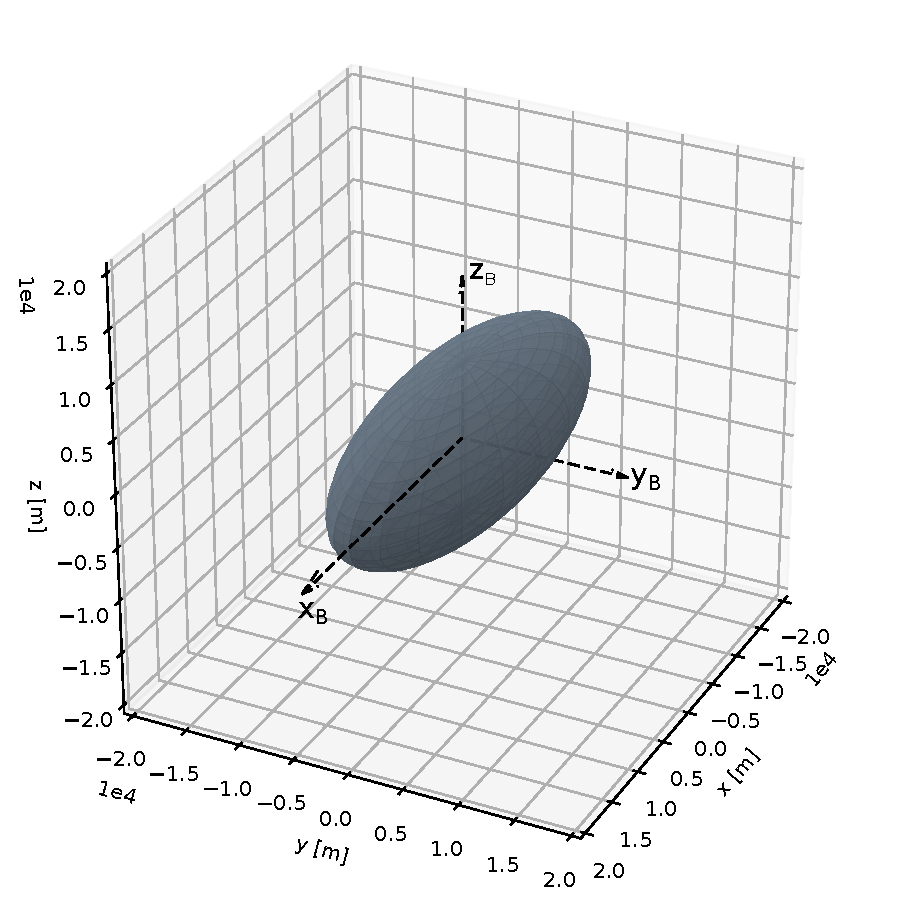
\includegraphics[width=\textwidth, height=0.35\textheight, keepaspectratio=true]{body_fixed_ellipsoid_frame.pdf}
\caption{Representation of the body-fixed rotating frame for a triaxial ellipsoid model of an asteroid. $\bm{x_{B}}$ is aligned with the longest axis, $\bm{z_{B}}$ is aligned with the shortest axis and $\bm{y_{B}}$ is aligned with the remaining last axis of the ellipsoid, satisfying the right-hand rule.}
\label{fig:ellipsoid_rotating_frame}
\end{figure}
\FloatBarrier
%%%
The two frames are defined as follows:
%%%
\begin{enumerate}
\item \gls{AIF} - This is a non-rotating frame fixed inertially in space with its origin at the centre of mass of the asteroid . \Cref{fig:solar_phase_and_inertial_frame} shows the orientation of the frame (in \emph{x-y} plane) such that the \emph{x-axis} is pointing to the Sun when the Longitude of the Sun (or effectively the True Anomaly of the apparent circular motion of the Sun around the asteroid) $\vartheta$ is zero. The \emph{y-axis}, thus, points to the sun when $\vartheta = 90^o$ and finally the \emph{z-axis} is obtained by following the right-hand rule, coming out of the sheet in 3D.
%
\item \gls{ARF} - This frame is fixed to the rotating asteroid with its origin at the centre of mass of the asteroid and axes aligned with the principle axes of the asteroid. \Cref{fig:ellipsoid_rotating_frame} shows the orientation of this frame, assuming a triaxial ellipsoid model for our asteroid (for details see \Cref{sec:gravity}). The \emph{x-axis} is pointing along the longest axis of the triaxial ellipsoid, and the \emph{z-axis} is pointing along the shortest axis of the ellipsoid. It is also aligned with the $z_I$ axis of \gls{AIF} as shown in \Cref{fig:reference_frame}. The \emph{y-axis} points in the direction of the remaining third axis, satisfying the right-hand rule. The asteroid (and effectively the \gls{ARF}) is rotating in a counter-clockwise sense, with respect to the \gls{AIF}, with constant angular velocity $\omega$ about the $z_B$ axis as depicted in \Cref{fig:reference_frame}.
\end{enumerate}
%%%
%%%
\begin{figure}[htb]
\centering
\captionsetup{justification=centering}
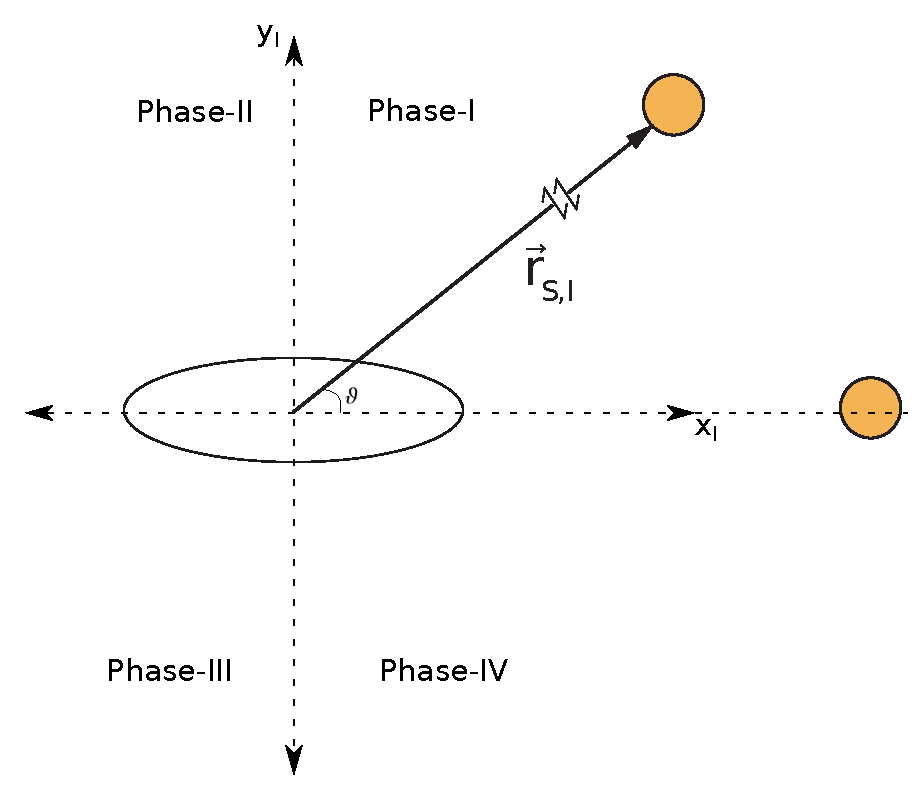
\includegraphics[width=\textwidth, height=0.35\textheight, keepaspectratio=true]{solar_phase_and_inertial_frame_3.pdf}
\caption{Asteroid-centric inertial frame \emph{x-y} plane. The position vector to the Sun is shown as $\protect\vv{\bm{r}}_{S,I}$. The apparent motion of the Sun around the asteroid, assumed a circular orbit, is also depicted with $\vartheta$ as the Longitude of Sun (or effectively the True Anomaly). The four phases are for a broader identification of the Sun's location with respect to the asteroid.}
\label{fig:solar_phase_and_inertial_frame}
\end{figure}
\FloatBarrier
%%%
We have two different frames of reference because it is important to visualize the same orbital motion with respect to both an inertial frame and a non-inertial frame to get a better understanding of the underlying dynamics. In this regard, it is thus important to be able to transfer a state vector between the two frames. The transfer matrix to transform a state vector from \gls{ARF} to \gls{AIF} is given as follows \parencite{schaub2003Book}:
%%%
\begin{equation}
    \begin{aligned}
        \phi_{B}^{I} &=
        \begin{bmatrix}
            \cos\theta & -\sin\theta & 0 \\
            \sin\theta & \cos\theta & 0 \\
            0 & 0 & 1
        \end{bmatrix}
        \\
        \theta &= \omega t
    \end{aligned}
    \label{eqn:arf_to_aif_transformation matrix}
\end{equation}
%%%
In \Cref{eqn:arf_to_aif_transformation matrix}, $\theta$ is the angle of rotation between the \gls{ARF} \& the \gls{AIF} at any given time $t$; and $\omega$ is the constant angular velocity of the rotating asteroid about $z_I / z_B$ axis as shown in \Cref{fig:reference_frame}. The position vector is then transformed, from \gls{ARF} to \gls{AIF}, as follows \parencite{schaub2003Book}:
%%%
\begin{align}
    \begin{bmatrix}
        x_I \\
        y_I \\
        z_I
    \end{bmatrix}
    =
    \begin{bmatrix}
        \cos\theta & -\sin\theta & 0 \\
        \sin\theta & \cos\theta & 0 \\
        0 & 0 & 1
    \end{bmatrix}
    \begin{bmatrix}
        x_B \\
        y_B \\
        z_B
    \end{bmatrix}
    \label{eqn:arf_to_aif_position_transformation}
\end{align}
%%%
In \Cref{eqn:arf_to_aif_position_transformation}, $x_I$ \& $x_B$ are the x-components of the position vector in \gls{AIF} and \gls{ARF} respectively; other components follow similar definitions. The velocity transformation takes place by first using the \textit{transport theorem} and then multiplying the resultant with the transformation matrix $\phi_{B}^{I}$ \parencite{schaub2003Book}. The transformation is shown as follows:
%%%
\begin{align}
    \vv{\bm{v}}_{I}^{B} &= \vv{\bm{v}}_{B} + \vv{\bm{\omega}} \times \vv{\bm{r}}_{B}
    \label{eqn:arf_to_aif_transport_theorem} \\
    \vv{\bm{v}}_I &= \phi_B^I \vv{\bm{v}}_I^B
    \label{eqn:arf_to_aif_velocity_transformation}
\end{align}
%%%
\Cref{eqn:arf_to_aif_transport_theorem} is the application of the transport theorem to get the \gls{AIF} velocity in \gls{ARF} components ($\vv{\bm{v}}_{I}^{B}$). In that, $\vv{\bm{v}}_{B}$ is the velocity vector in the \gls{ARF}, $\vv{\bm{\omega}}$ is the angular velocity vector for the asteroid's rotation (note that we have only uniform rotation about the $z_B$ axis), and $\vv{\bm{r}}_{B}$ is the position vector defined in the \gls{ARF}. In \Cref{eqn:arf_to_aif_velocity_transformation}, $\vv{\bm{v}}_I$ is the velocity vector in the \gls{AIF}.
%
\newline\newline
%
The transfer matrix to transform a state vector from \gls{AIF} to \gls{ARF} is just the transpose of $\phi_B^I$ as it is orthogonal \parencite{schaub2003Book}. It is given as follows:
%%%
\begin{align}
    \phi_{I}^{B} &=
    \begin{bmatrix}
        \cos\theta & \sin\theta & 0 \\
        -\sin\theta & \cos\theta & 0 \\
        0 & 0 & 1
    \end{bmatrix}
    \label{eqn:arf_to_aif_transformation matrix}
\end{align}
%%%


\section{Gravity Modeling}
\label{sec:gravity}
...elliptic integral method and how the accelerations are calculated and the third order equation solving for lambda...

\section{Solar Perturbations}
\label{sec:solar_perturbations}

\section{Perturbed Two-Body Problem}
\label{sec:2BP}

\section{Particle Initial Conditions}
\label{sec:init_conditions}
...launch velocity, location and direction calculation...

\section{Non-conservative Escape Speed}
\label{sec:escape_speed_derivation}

\section{Conclusion}
\label{sec:dynamics_conclusion}
